% 图 81.4 —— 由 `checks/emit_hand.py` 自动拼出（probe 精测 + prims2 图元分解）
%%
% ⚠ 这是**稿子不是成品**：跑 `checks/checkhand.py 81.4` 看指标 + 看叠合图。
%%
%% ⚠ 待核：
%   · 本图 probe 报出阴影族 1 个 —— **本脚本不生成阴影**（要照原书手写）；prims2 的 strokes 里可能含阴影线，核对时留意别画重
%   · 可疑字形 1 项（空心圈 ⊙ 常被认成字母 o）—— 见文件末
%%
\documentclass[12pt]{standalone}
\usepackage{fontspec}
\setsansfont{Arial}
\newfontfamily\mfallback{DejaVu Sans}
\usepackage{tikz}
\begin{document}
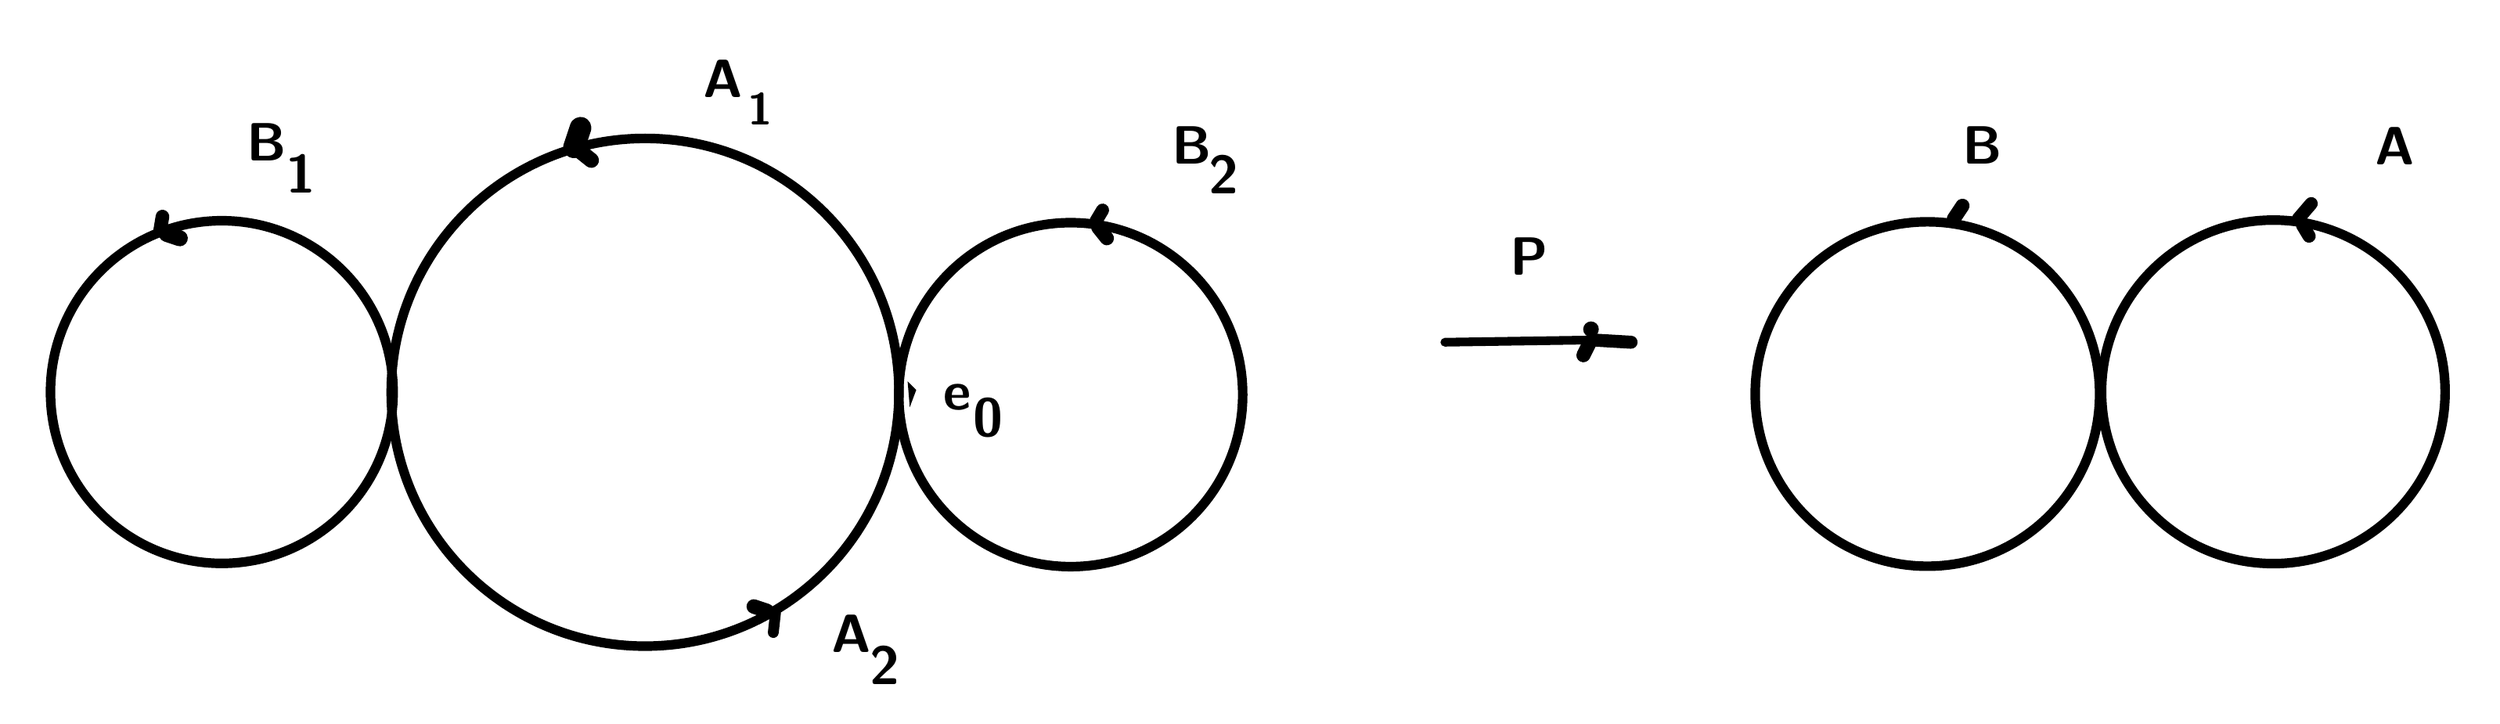
\begin{tikzpicture}[x=1pt, y=-1pt, line width=4.4pt, line cap=round, line join=round]

  %% ════ 填充区（prims2 的 fills）════
  \fill (409.0,166.0) -- (410.0,178.0) -- (413.0,170.0) -- cycle;

  %% ════ 直线段（prims2 的 strokes）════
  \draw[line width=6.5pt] (501.0,100.0) -- (497.0,95.0);
  \draw[line width=6.5pt] (724.0,148.0) -- (721.0,154.0);
  \draw[line width=6.7pt] (338.0,270.0) -- (344.0,272.0);
  \draw[line width=7.0pt] (263.0,64.0) -- (258.0,60.0);
  \draw[line width=5.0pt] (348.0,273.0) -- (347.0,282.0);
  \draw[line width=6.0pt] (1051.0,91.0) -- (1057.0,84.0);
  \draw[line width=10.0pt] (258.0,49.0) -- (255.0,58.0);
  \draw[line width=4.0pt] (657.0,148.0) -- (723.0,147.0);
  \draw[line width=7.4pt] (73.0,100.0) -- (67.0,98.0);
  \draw[line width=6.1pt] (1053.0,94.0) -- (1056.0,99.0);
  \draw[line width=6.0pt] (726.0,147.0) -- (743.0,148.0);
  \draw[line width=6.3pt] (64.0,96.0) -- (65.0,90.0);
  \draw[line width=6.0pt] (496.0,92.0) -- (499.0,87.0);
  \draw[line width=6.5pt] (892.0,91.0) -- (896.0,85.0);

  %% ════ 圆 / 椭圆（probe 精测）════
  \draw (287.8,171.1) circle (117.2);
  \draw (484.3,172.2) circle (79.4);
  \draw (879.8,171.9) circle (79.5);
  \draw (1039.5,170.9) circle (79.3);
  \draw (92.4,171.0) circle (79.1);

  %% ════ 实心点 ════
  \fill (724.5,142.0) circle (3.6);

  %% ════ 标签（probe 直接给的 \node 行）════
  %% ⚠ 全部补了 fill=white：文字在最上层，否则与曲线交叉干扰
     \node[anchor=center,inner sep=0pt,fill=white,font=\fontsize{30.3}{37.9}\selectfont] at (323.8,26.5) {\textsf{\textbf{\textit{A}}}};   % box(311,15,20,22)
     \node[anchor=center,inner sep=0pt,fill=white,font=\fontsize{22.2}{27.8}\selectfont] at (341.1,40.4) {\textsf{\textbf{1}}};   % box(335,32,7,16)
     \node[anchor=center,inner sep=0pt,fill=white,font=\fontsize{29.6}{37.0}\selectfont] at (113.2,55.5) {\textsf{\textbf{\textit{B}}}};   % box(102,44,19,22)
     \node[anchor=center,inner sep=0pt,fill=white,font=\fontsize{30.2}{37.8}\selectfont] at (540.3,57.0) {\textsf{\textbf{\textit{B}}}};   % box(529,45,19,23)
     \node[anchor=center,inner sep=0pt,fill=white,font=\fontsize{30.2}{37.8}\selectfont] at (905.3,57.0) {\textsf{\textbf{\textit{B}}}};   % box(894,45,19,23)
     \node[anchor=center,inner sep=0pt,fill=white,font=\fontsize{30.3}{37.9}\selectfont] at (1095.8,57.5) {\textsf{\textbf{\textit{A}}}};   % box(1083,46,20,22)
     \node[anchor=center,inner sep=0pt,fill=white,font=\fontsize{23.7}{29.7}\selectfont] at (128.8,70.4) {\textsf{\textbf{1}}};   % box(122,62,8,16)
     \node[anchor=center,inner sep=0pt,fill=white,font=\fontsize{23.6}{29.6}\selectfont] at (555.1,70.9) {\textsf{\textbf{2}}};   % box(549,62,11,17)
     \node[anchor=center,inner sep=0pt,fill=white,font=\fontsize{29.8}{37.3}\selectfont] at (696.0,108.5) {\textsf{\textbf{\textit{P}}}};   % box(685,96,18,23)
     \node[anchor=center,inner sep=0pt,fill=white,font=\fontsize{32.4}{40.5}\selectfont] at (431.9,173.6) {\textsf{\textbf{\textit{e}}}};   % box(422,163,16,18)
     \node[anchor=center,inner sep=0pt,fill=white,font=\fontsize{24.9}{31.1}\selectfont] at (446.1,182.7) {\textsf{\textbf{0}}};   % box(438,174,12,17)
     \node[anchor=center,inner sep=0pt,fill=white,font=\fontsize{29.6}{37.0}\selectfont] at (383.2,282.5) {\textsf{\textbf{\textit{A}}}};   % box(371,271,19,22)
     \node[anchor=center,inner sep=0pt,fill=white,font=\fontsize{24.0}{30.0}\selectfont] at (398.6,297.4) {\textsf{\textbf{2}}};   % box(392,289,12,16)

  % 钉死画布：否则超出的图元/控制点会把页面撑大，1:1 回比就失准
  \pgfresetboundingbox
  \path[use as bounding box] (0,0) rectangle (1134,314);
\end{tikzpicture}
\end{document}

% ⚠ 待核清单（probe 拿不准，人眼过一遍）：
%   · 未识别/跳过：⑤ 跳过/未识别的字形
